\documentclass[a4paper, 11pt]{article}
\usepackage{comment} % enables the use of multi-line comments (\ifx \fi) 
\usepackage{fullpage} % changes the margin
\usepackage[a4paper, total={7in, 10in}]{geometry}
\usepackage{amsmath,mathtools,mathdots}
\usepackage{amssymb,amsthm}  % assumes amsmath package installed
\usepackage{float}
\usepackage{xcolor}
\usepackage{mdframed}
\usepackage[shortlabels]{enumitem}
\usepackage{indentfirst}
\usepackage{hyperref}
\hypersetup{
	colorlinks=true,
	linkcolor=doc!80,
	citecolor=myr,
	filecolor=myr,      
	urlcolor=doc!80,
	pdftitle={Assignment}, %%%%%%%%%%%%%%%%   WRITE ASSIGNMENT PDF NAME  %%%%%%%%%%%%%%%%%%%%
}
\usepackage[most,many,breakable]{tcolorbox}
\usepackage{tikz}
\usepackage{caption}
\usepackage{mathpazo}
% Use the libertine package for the Libertine font
\usepackage{libertine}
\usepackage[libertine]{newtxmath}
\usepackage{libertine}
\usepackage{physics}
\usepackage[ruled,vlined,linesnumbered]{algorithm2e}
\usepackage{mathrsfs}
\usepackage{tikz-cd}
\usepackage{float}
\usepackage{pgfplots}
\definecolor{mytheorembg}{HTML}{F2F2F9}
\definecolor{mytheoremfr}{HTML}{00007B}
\definecolor{doc}{RGB}{0,60,110}
\definecolor{myg}{RGB}{56, 140, 70}
\definecolor{myb}{RGB}{45, 111, 177}
\definecolor{myr}{RGB}{199, 68, 64}

\usetikzlibrary{decorations.pathreplacing,angles,quotes,patterns}
\definecolor{mytheorembg}{HTML}{F2F2F9}
\definecolor{mytheoremfr}{HTML}{00007B}
\definecolor{doc}{RGB}{0,60,110}
\definecolor{myg}{RGB}{56, 140, 70}
\definecolor{myb}{RGB}{45, 111, 177}
\definecolor{myr}{RGB}{199, 68, 64}
\newcounter{problem}
\tcbuselibrary{theorems,skins,hooks}
\newtcbtheorem[use counter=problem]{problem}{Problem}
{%
	enhanced,
	breakable,
	colback = mytheorembg,
	frame hidden,
	boxrule = 0sp,
	borderline west = {2pt}{0pt}{mytheoremfr},
	arc=5pt,
	detach title,
	before upper = \tcbtitle\par\smallskip,
	coltitle = mytheoremfr,
	fonttitle = \bfseries\sffamily,
	description font = \mdseries,
	separator sign none,
	segmentation style={solid, mytheoremfr},
}
{p}

\newtheorem{lemma}{Lemma}
\renewenvironment{proof}{\noindent{\it \textbf{Proof:}}\hspace*{1em}}{\qed\bigskip\\}
% To give references for any problem use like this
% suppose the problem number is p3 then 2 options either 
% \hyperref[p:p3]{<text you want to use to hyperlink> \ref{p:p3}}
%                  or directly 
%                   \ref{p:p3}



%---------------------------------------
% BlackBoard Math Fonts :-
%---------------------------------------

%Captital Letters
\newcommand{\bbA}{\mathbb{A}}	\newcommand{\bbB}{\mathbb{B}}
\newcommand{\bbC}{\mathbb{C}}	\newcommand{\bbD}{\mathbb{D}}
\newcommand{\bbE}{\mathbb{E}}	\newcommand{\bbF}{\mathbb{F}}
\newcommand{\bbG}{\mathbb{G}}	\newcommand{\bbH}{\mathbb{H}}
\newcommand{\bbI}{\mathbb{I}}	\newcommand{\bbJ}{\mathbb{J}}
\newcommand{\bbK}{\mathbb{K}}	\newcommand{\bbL}{\mathbb{L}}
\newcommand{\bbM}{\mathbb{M}}	\newcommand{\bbN}{\mathbb{N}}
\newcommand{\bbO}{\mathbb{O}}	\newcommand{\bbP}{\mathbb{P}}
\newcommand{\bbQ}{\mathbb{Q}}	\newcommand{\bbR}{\mathbb{R}}
\newcommand{\bbS}{\mathbb{S}}	\newcommand{\bbT}{\mathbb{T}}
\newcommand{\bbU}{\mathbb{U}}	\newcommand{\bbV}{\mathbb{V}}
\newcommand{\bbW}{\mathbb{W}}	\newcommand{\bbX}{\mathbb{X}}
\newcommand{\bbY}{\mathbb{Y}}	\newcommand{\bbZ}{\mathbb{Z}}

%---------------------------------------
% MathCal Fonts :-
%---------------------------------------

%Captital Letters
\newcommand{\mcA}{\mathcal{A}}	\newcommand{\mcB}{\mathcal{B}}
\newcommand{\mcC}{\mathcal{C}}	\newcommand{\mcD}{\mathcal{D}}
\newcommand{\mcE}{\mathcal{E}}	\newcommand{\mcF}{\mathcal{F}}
\newcommand{\mcG}{\mathcal{G}}	\newcommand{\mcH}{\mathcal{H}}
\newcommand{\mcI}{\mathcal{I}}	\newcommand{\mcJ}{\mathcal{J}}
\newcommand{\mcK}{\mathcal{K}}	\newcommand{\mcL}{\mathcal{L}}
\newcommand{\mcM}{\mathcal{M}}	\newcommand{\mcN}{\mathcal{N}}
\newcommand{\mcO}{\mathcal{O}}	\newcommand{\mcP}{\mathcal{P}}
\newcommand{\mcQ}{\mathcal{Q}}	\newcommand{\mcR}{\mathcal{R}}
\newcommand{\mcS}{\mathcal{S}}	\newcommand{\mcT}{\mathcal{T}}
\newcommand{\mcU}{\mathcal{U}}	\newcommand{\mcV}{\mathcal{V}}
\newcommand{\mcW}{\mathcal{W}}	\newcommand{\mcX}{\mathcal{X}}
\newcommand{\mcY}{\mathcal{Y}}	\newcommand{\mcZ}{\mathcal{Z}}



%---------------------------------------
% Bold Math Fonts :-
%---------------------------------------

%Captital Letters
\newcommand{\bmA}{\boldsymbol{A}}	\newcommand{\bmB}{\boldsymbol{B}}
\newcommand{\bmC}{\boldsymbol{C}}	\newcommand{\bmD}{\boldsymbol{D}}
\newcommand{\bmE}{\boldsymbol{E}}	\newcommand{\bmF}{\boldsymbol{F}}
\newcommand{\bmG}{\boldsymbol{G}}	\newcommand{\bmH}{\boldsymbol{H}}
\newcommand{\bmI}{\boldsymbol{I}}	\newcommand{\bmJ}{\boldsymbol{J}}
\newcommand{\bmK}{\boldsymbol{K}}	\newcommand{\bmL}{\boldsymbol{L}}
\newcommand{\bmM}{\boldsymbol{M}}	\newcommand{\bmN}{\boldsymbol{N}}
\newcommand{\bmO}{\boldsymbol{O}}	\newcommand{\bmP}{\boldsymbol{P}}
\newcommand{\bmQ}{\boldsymbol{Q}}	\newcommand{\bmR}{\boldsymbol{R}}
\newcommand{\bmS}{\boldsymbol{S}}	\newcommand{\bmT}{\boldsymbol{T}}
\newcommand{\bmU}{\boldsymbol{U}}	\newcommand{\bmV}{\boldsymbol{V}}
\newcommand{\bmW}{\boldsymbol{W}}	\newcommand{\bmX}{\boldsymbol{X}}
\newcommand{\bmY}{\boldsymbol{Y}}	\newcommand{\bmZ}{\boldsymbol{Z}}
%Small Letters
\newcommand{\bma}{\boldsymbol{a}}	\newcommand{\bmb}{\boldsymbol{b}}
\newcommand{\bmc}{\boldsymbol{c}}	\newcommand{\bmd}{\boldsymbol{d}}
\newcommand{\bme}{\boldsymbol{e}}	\newcommand{\bmf}{\boldsymbol{f}}
\newcommand{\bmg}{\boldsymbol{g}}	\newcommand{\bmh}{\boldsymbol{h}}
\newcommand{\bmi}{\boldsymbol{i}}	\newcommand{\bmj}{\boldsymbol{j}}
\newcommand{\bmk}{\boldsymbol{k}}	\newcommand{\bml}{\boldsymbol{l}}
\newcommand{\bmm}{\boldsymbol{m}}	\newcommand{\bmn}{\boldsymbol{n}}
\newcommand{\bmo}{\boldsymbol{o}}	\newcommand{\bmp}{\boldsymbol{p}}
\newcommand{\bmq}{\boldsymbol{q}}	\newcommand{\bmr}{\boldsymbol{r}}
\newcommand{\bms}{\boldsymbol{s}}	\newcommand{\bmt}{\boldsymbol{t}}
\newcommand{\bmu}{\boldsymbol{u}}	\newcommand{\bmv}{\boldsymbol{v}}
\newcommand{\bmw}{\boldsymbol{w}}	\newcommand{\bmx}{\boldsymbol{x}}
\newcommand{\bmy}{\boldsymbol{y}}	\newcommand{\bmz}{\boldsymbol{z}}


%---------------------------------------
% Scr Math Fonts :-
%---------------------------------------

\newcommand{\sA}{{\mathscr{A}}}   \newcommand{\sB}{{\mathscr{B}}}
\newcommand{\sC}{{\mathscr{C}}}   \newcommand{\sD}{{\mathscr{D}}}
\newcommand{\sE}{{\mathscr{E}}}   \newcommand{\sF}{{\mathscr{F}}}
\newcommand{\sG}{{\mathscr{G}}}   \newcommand{\sH}{{\mathscr{H}}}
\newcommand{\sI}{{\mathscr{I}}}   \newcommand{\sJ}{{\mathscr{J}}}
\newcommand{\sK}{{\mathscr{K}}}   \newcommand{\sL}{{\mathscr{L}}}
\newcommand{\sM}{{\mathscr{M}}}   \newcommand{\sN}{{\mathscr{N}}}
\newcommand{\sO}{{\mathscr{O}}}   \newcommand{\sP}{{\mathscr{P}}}
\newcommand{\sQ}{{\mathscr{Q}}}   \newcommand{\sR}{{\mathscr{R}}}
\newcommand{\sS}{{\mathscr{S}}}   \newcommand{\sT}{{\mathscr{T}}}
\newcommand{\sU}{{\mathscr{U}}}   \newcommand{\sV}{{\mathscr{V}}}
\newcommand{\sW}{{\mathscr{W}}}   \newcommand{\sX}{{\mathscr{X}}}
\newcommand{\sY}{{\mathscr{Y}}}   \newcommand{\sZ}{{\mathscr{Z}}}


%---------------------------------------
% Math Fraktur Font
%---------------------------------------

%Captital Letters
\newcommand{\mfA}{\mathfrak{A}}	\newcommand{\mfB}{\mathfrak{B}}
\newcommand{\mfC}{\mathfrak{C}}	\newcommand{\mfD}{\mathfrak{D}}
\newcommand{\mfE}{\mathfrak{E}}	\newcommand{\mfF}{\mathfrak{F}}
\newcommand{\mfG}{\mathfrak{G}}	\newcommand{\mfH}{\mathfrak{H}}
\newcommand{\mfI}{\mathfrak{I}}	\newcommand{\mfJ}{\mathfrak{J}}
\newcommand{\mfK}{\mathfrak{K}}	\newcommand{\mfL}{\mathfrak{L}}
\newcommand{\mfM}{\mathfrak{M}}	\newcommand{\mfN}{\mathfrak{N}}
\newcommand{\mfO}{\mathfrak{O}}	\newcommand{\mfP}{\mathfrak{P}}
\newcommand{\mfQ}{\mathfrak{Q}}	\newcommand{\mfR}{\mathfrak{R}}
\newcommand{\mfS}{\mathfrak{S}}	\newcommand{\mfT}{\mathfrak{T}}
\newcommand{\mfU}{\mathfrak{U}}	\newcommand{\mfV}{\mathfrak{V}}
\newcommand{\mfW}{\mathfrak{W}}	\newcommand{\mfX}{\mathfrak{X}}
\newcommand{\mfY}{\mathfrak{Y}}	\newcommand{\mfZ}{\mathfrak{Z}}
%Small Letters
\newcommand{\mfa}{\mathfrak{a}}	\newcommand{\mfb}{\mathfrak{b}}
\newcommand{\mfc}{\mathfrak{c}}	\newcommand{\mfd}{\mathfrak{d}}
\newcommand{\mfe}{\mathfrak{e}}	\newcommand{\mff}{\mathfrak{f}}
\newcommand{\mfg}{\mathfrak{g}}	\newcommand{\mfh}{\mathfrak{h}}
\newcommand{\mfi}{\mathfrak{i}}	\newcommand{\mfj}{\mathfrak{j}}
\newcommand{\mfk}{\mathfrak{k}}	\newcommand{\mfl}{\mathfrak{l}}
\newcommand{\mfm}{\mathfrak{m}}	\newcommand{\mfn}{\mathfrak{n}}
\newcommand{\mfo}{\mathfrak{o}}	\newcommand{\mfp}{\mathfrak{p}}
\newcommand{\mfq}{\mathfrak{q}}	\newcommand{\mfr}{\mathfrak{r}}
\newcommand{\mfs}{\mathfrak{s}}	\newcommand{\mft}{\mathfrak{t}}
\newcommand{\mfu}{\mathfrak{u}}	\newcommand{\mfv}{\mathfrak{v}}
\newcommand{\mfw}{\mathfrak{w}}	\newcommand{\mfx}{\mathfrak{x}}
\newcommand{\mfy}{\mathfrak{y}}	\newcommand{\mfz}{\mathfrak{z}}

%---------------------------------------
% Bar
%---------------------------------------

%Captital Letters
\newcommand{\ovA}{\overline{A}}	\newcommand{\ovB}{\overline{B}}
\newcommand{\ovC}{\overline{C}}	\newcommand{\ovD}{\overline{D}}
\newcommand{\ovE}{\overline{E}}	\newcommand{\ovF}{\overline{F}}
\newcommand{\ovG}{\overline{G}}	\newcommand{\ovH}{\overline{H}}
\newcommand{\ovI}{\overline{I}}	\newcommand{\ovJ}{\overline{J}}
\newcommand{\ovK}{\overline{K}}	\newcommand{\ovL}{\overline{L}}
\newcommand{\ovM}{\overline{M}}	\newcommand{\ovN}{\overline{N}}
\newcommand{\ovO}{\overline{O}}	\newcommand{\ovP}{\overline{P}}
\newcommand{\ovQ}{\overline{Q}}	\newcommand{\ovR}{\overline{R}}
\newcommand{\ovS}{\overline{S}}	\newcommand{\ovT}{\overline{T}}
\newcommand{\ovU}{\overline{U}}	\newcommand{\ovV}{\overline{V}}
\newcommand{\ovW}{\overline{W}}	\newcommand{\ovX}{\overline{X}}
\newcommand{\ovY}{\overline{Y}}	\newcommand{\ovZ}{\overline{Z}}
%Small Letters
\newcommand{\ova}{\overline{a}}	\newcommand{\ovb}{\overline{b}}
\newcommand{\ovc}{\overline{c}}	\newcommand{\ovd}{\overline{d}}
\newcommand{\ove}{\overline{e}}	\newcommand{\ovf}{\overline{f}}
\newcommand{\ovg}{\overline{g}}	\newcommand{\ovh}{\overline{h}}
\newcommand{\ovi}{\overline{i}}	\newcommand{\ovj}{\overline{j}}
\newcommand{\ovk}{\overline{k}}	\newcommand{\ovl}{\overline{l}}
\newcommand{\ovm}{\overline{m}}	\newcommand{\ovn}{\overline{n}}
\newcommand{\ovo}{\overline{o}}	\newcommand{\ovp}{\overline{p}}
\newcommand{\ovq}{\overline{q}}	\newcommand{\ovr}{\overline{r}}
\newcommand{\ovs}{\overline{s}}	\newcommand{\ovt}{\overline{t}}
\newcommand{\ovu}{\overline{u}}	\newcommand{\ovv}{\overline{v}}
\newcommand{\ovw}{\overline{w}}	\newcommand{\ovx}{\overline{x}}
\newcommand{\ovy}{\overline{y}}	\newcommand{\ovz}{\overline{z}}

%---------------------------------------
% Tilde
%---------------------------------------

%Captital Letters
\newcommand{\tdA}{\tilde{A}}	\newcommand{\tdB}{\tilde{B}}
\newcommand{\tdC}{\tilde{C}}	\newcommand{\tdD}{\tilde{D}}
\newcommand{\tdE}{\tilde{E}}	\newcommand{\tdF}{\tilde{F}}
\newcommand{\tdG}{\tilde{G}}	\newcommand{\tdH}{\tilde{H}}
\newcommand{\tdI}{\tilde{I}}	\newcommand{\tdJ}{\tilde{J}}
\newcommand{\tdK}{\tilde{K}}	\newcommand{\tdL}{\tilde{L}}
\newcommand{\tdM}{\tilde{M}}	\newcommand{\tdN}{\tilde{N}}
\newcommand{\tdO}{\tilde{O}}	\newcommand{\tdP}{\tilde{P}}
\newcommand{\tdQ}{\tilde{Q}}	\newcommand{\tdR}{\tilde{R}}
\newcommand{\tdS}{\tilde{S}}	\newcommand{\tdT}{\tilde{T}}
\newcommand{\tdU}{\tilde{U}}	\newcommand{\tdV}{\tilde{V}}
\newcommand{\tdW}{\tilde{W}}	\newcommand{\tdX}{\tilde{X}}
\newcommand{\tdY}{\tilde{Y}}	\newcommand{\tdZ}{\tilde{Z}}
%Small Letters
\newcommand{\tda}{\tilde{a}}	\newcommand{\tdb}{\tilde{b}}
\newcommand{\tdc}{\tilde{c}}	\newcommand{\tdd}{\tilde{d}}
\newcommand{\tde}{\tilde{e}}	\newcommand{\tdf}{\tilde{f}}
\newcommand{\tdg}{\tilde{g}}	\newcommand{\tdh}{\tilde{h}}
\newcommand{\tdi}{\tilde{i}}	\newcommand{\tdj}{\tilde{j}}
\newcommand{\tdk}{\tilde{k}}	\newcommand{\tdl}{\tilde{l}}
\newcommand{\tdm}{\tilde{m}}	\newcommand{\tdn}{\tilde{n}}
\newcommand{\tdo}{\tilde{o}}	\newcommand{\tdp}{\tilde{p}}
\newcommand{\tdq}{\tilde{q}}	\newcommand{\tdr}{\tilde{r}}
\newcommand{\tds}{\tilde{s}}	\newcommand{\tdt}{\tilde{t}}
\newcommand{\tdu}{\tilde{u}}	\newcommand{\tdv}{\tilde{v}}
\newcommand{\tdw}{\tilde{w}}	\newcommand{\tdx}{\tilde{x}}
\newcommand{\tdy}{\tilde{y}}	\newcommand{\tdz}{\tilde{z}}

%---------------------------------------
% Vec
%---------------------------------------

%Captital Letters
\newcommand{\vcA}{\vec{A}}	\newcommand{\vcB}{\vec{B}}
\newcommand{\vcC}{\vec{C}}	\newcommand{\vcD}{\vec{D}}
\newcommand{\vcE}{\vec{E}}	\newcommand{\vcF}{\vec{F}}
\newcommand{\vcG}{\vec{G}}	\newcommand{\vcH}{\vec{H}}
\newcommand{\vcI}{\vec{I}}	\newcommand{\vcJ}{\vec{J}}
\newcommand{\vcK}{\vec{K}}	\newcommand{\vcL}{\vec{L}}
\newcommand{\vcM}{\vec{M}}	\newcommand{\vcN}{\vec{N}}
\newcommand{\vcO}{\vec{O}}	\newcommand{\vcP}{\vec{P}}
\newcommand{\vcQ}{\vec{Q}}	\newcommand{\vcR}{\vec{R}}
\newcommand{\vcS}{\vec{S}}	\newcommand{\vcT}{\vec{T}}
\newcommand{\vcU}{\vec{U}}	\newcommand{\vcV}{\vec{V}}
\newcommand{\vcW}{\vec{W}}	\newcommand{\vcX}{\vec{X}}
\newcommand{\vcY}{\vec{Y}}	\newcommand{\vcZ}{\vec{Z}}
%Small Letters
\newcommand{\vca}{\vec{a}}	\newcommand{\vcb}{\vec{b}}
\newcommand{\vcc}{\vec{c}}	\newcommand{\vcd}{\vec{d}}
\newcommand{\vce}{\vec{e}}	\newcommand{\vcf}{\vec{f}}
\newcommand{\vcg}{\vec{g}}	\newcommand{\vch}{\vec{h}}
\newcommand{\vci}{\vec{i}}	\newcommand{\vcj}{\vec{j}}
\newcommand{\vck}{\vec{k}}	\newcommand{\vcl}{\vec{l}}
\newcommand{\vcm}{\vec{m}}	\newcommand{\vcn}{\vec{n}}
\newcommand{\vco}{\vec{o}}	\newcommand{\vcp}{\vec{p}}
\newcommand{\vcq}{\vec{q}}	\newcommand{\vcr}{\vec{r}}
\newcommand{\vcs}{\vec{s}}	\newcommand{\vct}{\vec{t}}
\newcommand{\vcu}{\vec{u}}	\newcommand{\vcv}{\vec{v}}
%\newcommand{\vcw}{\vec{w}}	\newcommand{\vcx}{\vec{x}}
\newcommand{\vcy}{\vec{y}}	\newcommand{\vcz}{\vec{z}}

%---------------------------------------
% Greek Letters:-
%---------------------------------------
\newcommand{\eps}{\epsilon}
\newcommand{\veps}{\varepsilon}
\newcommand{\lm}{\lambda}
\newcommand{\Lm}{\Lambda}
\newcommand{\gm}{\gamma}
\newcommand{\Gm}{\Gamma}
\newcommand{\vph}{\varphi}
\newcommand{\ph}{\phi}
\newcommand{\om}{\omega}
\newcommand{\Om}{\Omega}
\newcommand{\sg}{\sigma}
\newcommand{\Sg}{\Sigma}

\newcommand{\Qed}{\begin{flushright}\qed\end{flushright}}
\newcommand{\parinn}{\setlength{\parindent}{1cm}}
\newcommand{\parinf}{\setlength{\parindent}{0cm}}
\newcommand{\del}[2]{\frac{\partial #1}{\partial #2}}
\newcommand{\Del}[3]{\frac{\partial^{#1} #2}{\partial^{#1} #3}}
\newcommand{\deld}[2]{\dfrac{\partial #1}{\partial #2}}
\newcommand{\Deld}[3]{\dfrac{\partial^{#1} #2}{\partial^{#1} #3}}
\newcommand{\uin}{\mathbin{\rotatebox[origin=c]{90}{$\in$}}}
\newcommand{\usubset}{\mathbin{\rotatebox[origin=c]{90}{$\subset$}}}
\newcommand{\lt}{\left}
\newcommand{\rt}{\right}
\newcommand{\exs}{\exists}
\newcommand{\st}{\strut}
\newcommand{\dps}[1]{\displaystyle{#1}}
\newcommand{\la}{\langle}
\newcommand{\ra}{\rangle}
\newcommand{\cls}[1]{\textsc{#1}}
\newcommand{\prb}[1]{\textsc{#1}}
\newcommand{\comb}[2]{\left(\begin{matrix}
		#1\\ #2
\end{matrix}\right)}
%\newcommand[2]{\quotient}{\faktor{#1}{#2}}
\newcommand\quotient[2]{
	\mathchoice
	{% \displaystyle
		\text{\raise1ex\hbox{$#1$}\Big/\lower1ex\hbox{$#2$}}%
	}
	{% \textstyle
		#1\,/\,#2
	}
	{% \scriptstyle
		#1\,/\,#2
	}
	{% \scriptscriptstyle  
		#1\,/\,#2
	}
}

\newcommand{\tensor}{\otimes}
\newcommand{\xor}{\oplus}

\newcommand{\sol}[1]{\begin{solution}#1\end{solution}}
\newcommand{\solve}[1]{\setlength{\parindent}{0cm}\textbf{\textit{Solution: }}\setlength{\parindent}{1cm}#1 \hfill $\blacksquare$}
\newcommand{\mat}[1]{\left[\begin{matrix}#1\end{matrix}\right]}
\newcommand{\matr}[1]{\begin{matrix}#1\end{matrix}}
\newcommand{\matp}[1]{\lt(\begin{matrix}#1\end{matrix}\rt)}
\newcommand{\detmat}[1]{\lt|\begin{matrix}#1\end{matrix}\rt|}
\newcommand\numberthis{\addtocounter{equation}{1}\tag{\theequation}}
\newcommand{\handout}[3]{
	\noindent
	\begin{center}
		\framebox{
			\vbox{
				\hbox to 6.5in { {\bf Complexity Theory I } \hfill Jan -- May, 2023 }
				\vspace{4mm}
				\hbox to 6.5in { {\Large \hfill #1  \hfill} }
				\vspace{2mm}
				\hbox to 6.5in { {\em #2 \hfill #3} }
			}
		}
	\end{center}
	\vspace*{4mm}
}

\newcommand{\lecture}[3]{\handout{Lecture #1}{Lecturer: #2}{Scribe:	#3}}

\let\marvosymLightning\Lightning
\newcommand{\ctr}{\text{\marvosymLightning}\hspace{0.5ex}} % Requires marvosym package

\newcommand{\ov}[1]{\overline{#1}}
\newcommand{\thmref}[1]{\hyperref[th:#1]{Theorem \ref{th:#1}}}
\newcommand{\propref}[1]{\hyperref[th:#1]{Proposition \ref{th:#1}}}
\newcommand{\lmref}[1]{\hyperref[th:#1]{Lemma \ref{th:#1}}}
\newcommand{\corref}[1]{\hyperref[th:#1]{Corollary \ref{th:#1}}}

\newcommand{\thrmref}[1]{\hyperref[#1]{Theorem \ref{#1}}}
\newcommand{\propnref}[1]{\hyperref[#1]{Proposition \ref{#1}}}
\newcommand{\lemref}[1]{\hyperref[#1]{Lemma \ref{#1}}}
\newcommand{\corrref}[1]{\hyperref[#1]{Corollary \ref{#1}}}

\DeclareMathOperator{\enc}{Enc}
\DeclareMathOperator{\res}{Res}
\DeclareMathOperator{\spec}{Spec}
\DeclareMathOperator{\cov}{Cov}
\DeclareMathOperator{\Var}{Var}
\DeclareMathOperator{\Rank}{rank}
\newcommand{\Tfae}{The following are equivalent:}
\newcommand{\tfae}{the following are equivalent:}
\newcommand{\sparsity}{\textit{sparsity}}

\newcommand{\uddots}{\reflectbox{$\ddots$}} 

\newenvironment{claimwidth}{\begin{center}\begin{adjustwidth}{0.05\textwidth}{0.05\textwidth}}{\end{adjustwidth}\end{center}}

\setlength{\parindent}{0pt}

%%%%%%%%%%%%%%%%%%%%%%%%%%%%%%%%%%%%%%%%%%%%%%%%%%%%%%%%%%%%%%%%%%%%%%%%%%%%%%%%%%%%%%%%%%%%%%%%%%%%%%%%%%%%%%%%%%%%%%%%%%%%%%%%%%%%%%%%

\begin{document}
	
	%%%%%%%%%%%%%%%%%%%%%%%%%%%%%%%%%%%%%%%%%%%%%%%%%%%%%%%%%%%%%%%%%%%%%%%%%%%%%%%%%%%%%%%%%%%%%%%%%%%%%%%%%%%%%%%%%%%%%%%%%%%%%%%%%%%%%%%%
	
	\textsf{\noindent \large\textbf{Soham Chatterjee} \hfill \textbf{Assignment - 2}\\
		Email: \href{soham.chatterjee@tifr.res.in}{soham.chatterjee@tifr.res.in} \hfill Dept: STCS\\
		\normalsize Course: Probability Theory \hfill Date: \today}
	
%%%%%%%%%%%%%%%%%%%%%%%%%%%%%%%%%%%%%%%%%%%%%%%%%%%%%%%%%%%%%%%%%%%%%%%%%%%%%%%%%%%%%%%%%%%%%%%%%%%%%%%%%%%%%%%%%%%%%%%%%%%%%%%%%%%%%%%%
% Problem 1
%%%%%%%%%%%%%%%%%%%%%%%%%%%%%%%%%%%%%%%%%%%%%%%%%%%%%%%%%%%%%%%%%%%%%%%%%%%%%%%%%%%%%%%%%%%%%%%%%%%%%%%%%%%%%%%%%%%%%%%%%%%%%%%%%%%%%%%%
	
\begin{problem}{%problem statement
		[H] Problem 1.3: Ordering of three random variables
	}{p1% problem reference text
}
Suppose $X,Y$ and $U$ are mutually independent, such that $X$ and $Y$ are each exponentially distributed with some common parameter $\lm>0$ and $U$ is uniformly distributed on the interval $[0,1]$. Express $\bbP\{X<U<Y\}$ in terms of $\lm$. Simplify your answer.
\end{problem}
\solve{
$X$ and $Y$ are exponentially distributed with some common parameter $\lm>0$. Hence $F_X(x)=1- e^{-\lm x}$ and $F_Y(y)=1- e^{-\lm y}$ for some $x,y\geq 0$.and $U$ is uniform on $[0,1]$. So \begin{align*}
	\bbP[X<U<Y] & =\int_0^1\bbP[X< u, Y>u]du\\
	& = \int_0^1\bbP[X<u]\cdot \bbP[Y>u]du\\
	& = \int_0^1F_X(u)(1-F_Y(u))du\\
	& = \int_0^1 \lt(1-e^{-\lm u}\rt)\lt(1-\lt(1-e^{\lm u}\rt)\rt)du\\
	& = \int_0^1\lt(1-e^{-\lm u}\rt)e^{-\lm u}du\\
	& = \int_0^1 \lt[e^{-\lm u}-e^{-2\lm u}\rt]du\\
	& = \lt[\frac{e^{-\lm u}}{-\lm}-\frac{e^{-2\lm u}}{-2\lm}\rt]_0^1\\
	& = \lt[\frac{e^{-2\lm }}{2\lm}-\frac{e^{-\lm }}{\lm}\rt]-\lt[\frac{1}{2\lm}-\frac{1}{\lm}\rt] = \frac{\lt(e^{-\lm}\rt)^2-2e^{-\lm}+1}{2\lm}= \frac{\lt(e^{-\lm}-1\rt)^2}{2\lm}
\end{align*}
}
%%%%%%%%%%%%%%%%%%%%%%%%%%%%%%%%%%%%%%%%%%%%%%%%%%%%%%%%%%%%%%%%%%%%%%%%%%%%%%%%%%%%%%%%%%%%%%%%%%%%%%%%%%%%%%%%%%%%%%%%%%%%%%%%%%%%%%%%
% Problem 2
%%%%%%%%%%%%%%%%%%%%%%%%%%%%%%%%%%%%%%%%%%%%%%%%%%%%%%%%%%%%%%%%%%%%%%%%%%%%%%%%%%%%%%%%%%%%%%%%%%%%%%%%%%%%%%%%%%%%%%%%%%%%%%%%%%%%%%%%

\begin{problem}{%problem statement
		[H] Problem 1.5: Congestion at output ports
	}{p2% problem reference text
	}
Consider a packet switch with some number
of input ports and eight output ports. Suppose four packets simultaneously arrive
on different input ports, and each is routed toward an output port. Assume the
choices of output ports are mutually independent, and for each packet, each
output port has equal probability.\begin{enumerate}[label=(\alph*)]
	\item Specify a probability space $(\Om,\mcF,\bbP)$ to describe this situation.
	\item Let $X_i$ denote the number of packets routed to output port $i$ for $1\leq i\leq 8$. Describe the joint pmf of $X_1,\dots,X_8$.
	\item Find $\cov(X_1,X_2)$
	\item Find $\bbP[X_i\leq 1 \text{ for all $i$}]$
	\item Find $\bbP[X_i\leq 2 \text{ for all $i$}]$
\end{enumerate}
\end{problem}
\solve{
\begin{enumerate}[label=(\alph*)]
	\item Since each packet can be routed toward any of the $8$ output ports we keep all possible $4-$tuples in the sample space i.e. $$\Om = \{(\sg_1,\sg_2,\sg_3,\sg_4)\mid \sg_i\in[8] \ \forall\ i\in[4]\}$$Then we take $\mcF$ to be the power set of $\Om$, $\mcP(\Om)$ and the probability measure $\bbP$ is uniform i.e. for any $k_1,\dots, k_4\in [8]$  we have $$\bbP[(\sg_1,\sg_2,\sg_3,\sg_4)=(k_1,k_2,k_3,k_4)]=\frac1{8^4}$$Hence we have $\Om=\{1,\dots, 8\}^4$, $\mcF=\mcP(\Om)$ and $\bbP[\om]=\frac1{8^4}$ for each $\om\in \Om$.
	\item The random variables $X_i$ for $i\in[8]$ satisfy the following property $$X_1+X_2+\cdots+X_8=4$$Hence $$\bbP[X_1=x_1,\dots, X_8=x_8]=\frac1{8^4}\prod_{i=1}^8\matp{4-\sum\limits_{j=1}^{i-1}x_j \\ x_i}$$
	\item Now $$\bbP[X_k=i]=\dfrac{\binom{4}{i}7^{4-i}}{8^4}\text{ and } \bbP[X_k=i,X_l=j]=\dfrac{\binom{4}{i}\binom{4-i}{j}6^{4-(i+j)}}{8^4}$$Therefore we have $X_k\sim Bin\lt(4,\frac18\rt)$ for all $k\in[8]$. Hence $\bbE[X_k]=\frac{4}8=\frac12$ and $\Var[X_k]=4\frac18\frac78=\frac7{16}$. Therefore $\bbE[X_k^2]=\Var[X_k]+\bbE[X_k]^2=\frac7{16}+\frac14=\frac{11}{16}$ And also we have $$\bbP[X_l=j\mid X_k=i]=\frac{\binom{4-i}{j}6^{4-(i+j)}}{7^4}=\binom{4-i}{j}\lt(\frac{6}{7}\rt)^{4-(i+j)}\frac{1}{7^j}$$Therefore $(X_l\mid X_k=i)\sim Bin\lt(4-i,\frac17 \rt)$. Hence $\bbE[X_l\mid X_k=i]=\frac{4-i}7$. Now we will calculate the covariance.
	\begin{align*}
		\cov(X_1,X_2) & = \bbE[X_1X_2]-\bbE[X_1]\bbE[X_2]\\
		& = \bbE\lt[\bbE[X_1X_2\mid X_1]\rt]-\frac14\\
		& = \bbE\lt[   X_1\bbE[X_2\mid X_1]\rt]-\frac14\\
		& = \bbE\lt[X_1\frac{4-X_1}{7}\rt]-\frac14\\
		& = \bbE\lt[\frac{4X_1-X_1^2}7\rt]-\frac14\\
		& = \frac47\bbE[X_1]-\frac17\bbE[X_1^2]-\frac14\\
		& = \frac47 \frac12-\frac17 \frac{11}{16}-\frac14=-\frac1{16}
	\end{align*}

[I discussed with Spandan]
\item For all $i\in[8]$ we have \begin{align*}
	\bbP[X_i\leq 1] & = \bbP[X_i=0]+\bbP[X_i=1]\\
	& = \frac{\binom{4}{0}7^{4-0}}{8^4}+\frac{\binom{4}{1}7^{4-1}}{8^4}\\
	& = \frac{ 7^4}{8^4}+\frac{4\times 7^3}{8^4}=\frac{7^3\times 11}{8^4}
\end{align*}
\item For all $i\in[8]$ we have \begin{align*}
	\bbP[X_i\leq 2] & = 1-\bbP[X_i=3]-\bbP[X_i=4]\\
	& = 1-\frac{\binom{4}{3}7^{4-3}}{8^4}-\frac{\binom{4}{4}7^{4-4}}{8^4}\\
	& = 1-\frac{4\times 7}{8^4}-\frac{1}{8^4}=1-\frac{29}{8^4}
\end{align*}

\end{enumerate}

}

%%%%%%%%%%%%%%%%%%%%%%%%%%%%%%%%%%%%%%%%%%%%%%%%%%%%%%%%%%%%%%%%%%%%%%%%%%%%%%%%%%%%%%%%%%%%%%%%%%%%%%%%%%%%%%%%%%%%%%%%%%%%%%%%%%%%%%%%
% Problem 3
%%%%%%%%%%%%%%%%%%%%%%%%%%%%%%%%%%%%%%%%%%%%%%%%%%%%%%%%%%%%%%%%%%%%%%%%%%%%%%%%%%%%%%%%%%%%%%%%%%%%%%%%%%%%%%%%%%%%%%%%%%%%%%%%%%%%%%%%

\begin{problem}{%problem statement
		[H] Problem 1.13: A CDF of mixed type
	}{p3% problem reference text
	}
Let $X$ have the CDF shown.

\begin{center}
	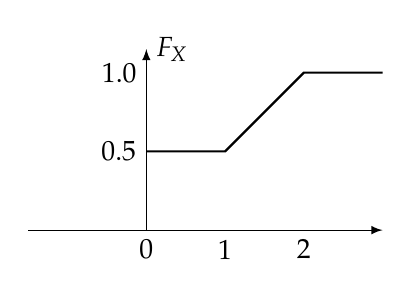
\begin{tikzpicture}
		\draw[-latex] (-1.5,0) -- (1,0) node[below] {$1$} -- (2,0) node[below]{$2$} -- (3,0);
		\draw[-latex] (0,0) node[below] {$0$} -- (0,2.3) node[above, right]{$F_X$};
		\draw[thick] (0,1) node[left] {$0.5$} -- (1,1) -- (2,2) -- (3,2); 
		\draw (0,2) node[left] {1.0};
	\end{tikzpicture}
\end{center}
\begin{enumerate}[label=(\alph*)]
	\item Find $\bbP[X\leq 0.8]$
	\item Find $\bbE[X]$
	\item Find $\Var [X]$
\end{enumerate}
\end{problem}
\solve{
\begin{enumerate}[label=(\alph*)]
	\item $\bbP[X\leq 0.8]=\bbF_X[0.8]=0.5$ since the value of $F_X$ increases when $X\geq 1$. 
	\item $F_X(x)=\begin{cases}
		0&\text{when $x\leq 0$}\\
		0.5 & \text{when} 0\leq x\leq 1\\
		0.5+\frac{x-1}2 & \text{when } 1\leq x\leq 2\\
		1& \text{when }x\geq 2
	\end{cases}$ 

Hence \begin{align*}
	\bbE[X]& =\int_0^{\infty}[1-F_X(x)]dx=\int_0^1[1-0.5]dx+\int_1^2\lt[1-0.5-\frac{x-1}2\rt]dx+\int_2^{\infty}[1-1]dx\\
	& =\int_0^10.5dx+\int_1^2\lt[0.5-\frac{x-1}2\rt]dx\\
	& = 0.5+\lt[0.5x-\frac{(x-1)^2}{4}\rt]^2_1= 1-\frac14=\frac34
\end{align*}
	\item Take $Y=X^2$ and the distribution function for $Y$ is $F_Y$. Now for any $y\geq 0$ $$F_Y(y)=\bbP[Y^2\leq y]=\bbP[X^2\leq y]=\bbP[X\leq \sqrt{y}]=F_X(\sqrt{y})$$
	Therefore $$F_Y(y)=\begin{cases}
		0&\text{when $x\leq 0$}\\
		0.5 & \text{when} 0\leq x\leq 1\\
		0.5+\frac{\sqrt{y}-1}2 & \text{when } 1\leq y\leq 4\\
		1& \text{when }y\geq 4
	\end{cases}$$Hence \begin{align*}
	\bbE[X^2] &  =\int_0^{\infty}[1-F_Y(y)]dy=\int_0^1[1-0.5]dy+\int_1^4\lt[1-0.5-\frac{\sqrt{y}-1}2\rt]dy+\int_4^{\infty}[1-1]dy\\
	& = \int_0^10.5dy+\int_1^4\lt[0.5-\frac{\sqrt{y}-1}{2}\rt]dy\\
	& = 0.5+\lt[ 0.5y-\frac{\frac23y^{\frac32}-y}{2} \rt]_1^4=0.5+3\cdot 0.5-\lt[ \frac{\frac234^{\frac32}-4}{2} - \frac{\frac231^{\frac32}-1}{2}\rt] =2 -\frac56=\frac{7}6
\end{align*}
So $\Var[X]=\bbE[X^2]-\bbE[X]=\frac{7}{6}-\frac9{16}=\frac{56-27}{48}=\frac{29}{48}$. 
\end{enumerate}
}

%%%%%%%%%%%%%%%%%%%%%%%%%%%%%%%%%%%%%%%%%%%%%%%%%%%%%%%%%%%%%%%%%%%%%%%%%%%%%%%%%%%%%%%%%%%%%%%%%%%%%%%%%%%%%%%%%%%%%%%%%%%%%%%%%%%%%%%%
% Problem 4
%%%%%%%%%%%%%%%%%%%%%%%%%%%%%%%%%%%%%%%%%%%%%%%%%%%%%%%%%%%%%%%%%%%%%%%%%%%%%%%%%%%%%%%%%%%%%%%%%%%%%%%%%%%%%%%%%%%%%%%%%%%%%%%%%%%%%%%%

\begin{problem}{%problem statement 
		[H] Problem 1.17: Transformation of a random variable
	}{p4% problem reference text
	}
Let $X$ be exponentially distributed with mean $\lm^{-1}$. Find and carefully sketch  distribution functions for the random variables $Y=\exp(X)$ and $Z=\min(X,3)$
\end{problem}
\solve{
	$X$ is exponentially distributed with mean $\lm^{-1}$. So the density function of $X$ for $x\geq 0$ is  $f\st_X(x)=\lm e^{-\lm x} $. So for $y> 0$, $$F\st_Y(y)=\bbP[Y\leq y]=\bbP[e^x\leq y]=\bbP[x\leq \ln y]=F\st_X[\ln y]=1-e^{-\lm [\ln y]}=1-\lt[e^{\ln y}\rt]^{-\lm}=1-y^{-\lm}$$
	
\begin{center}
%\begin{tikzpicture}[xscale=0.08,yscale=0.09,domain=0.140:60,samples=800]
\begin{tikzpicture}
	\begin{axis}[
		domain=1:23, % Define the x-range from 1 to 5
		samples=100, % Number of samples for a smooth curve
		xlabel=$Z$,
		ylabel={$F_Z(y)$},
		axis lines=middle,
		ymin=-0.2, ymax=1.2, % Set y-axis limits for a clear view
		xmin=-1, xmax=23, % Extend the x-axis from -1 to 6
		xtick={1,5,10,15,20}, % X-axis tick only at x=1
		thick
		]
		\addplot[
		red
		] {1 - x^(-1)}; % This plots 1 - x^{-2}
		\addplot[dashed] coordinates {(0, 1) (23, 1)};
		
		% Add the lambda text near the end of the graph
		\node at (axis cs:18, 1) [yshift=-0.5cm] {$\lambda = 1$};
	\end{axis}
\end{tikzpicture}
\end{center}
And for $z\geq 0$ $Z$ can be either equal to $X$ or $3$. $$F\st_Z(z)=\bbP[Z\leq z]=\bbP[\min({X,3})\leq z]$$Now there will be two cases. $z<3$ and $z\geq 3$. For $z<3$ $$F\st_Z(z)=\bbP[Z\leq z]=\bbP[X\leq z]=F\st_X(z)$$For $z\geq 3$ $$F\st_Z(z)=\bbP[Z\leq z]=\bbP[\{Z<3\} \cup\{Z=3\}]=\bbP[Z<3]+\bbP[Z\geq 3]=\bbP[X<3]+\bbP[X\geq 3]=F\st_X(3)+\lt[1-F\st_X(3)\rt]=1$$
\begin{center}
\begin{tikzpicture}
	\begin{axis}[
		domain=0:5, % Set the x-range from 0 to 5
		samples=100, % Number of samples for smooth curve
		xlabel=$Y$,
		ylabel={$F_Y(y)$},
		axis lines=middle,
		xtick={-1,0,1,2,3,4}, % X-axis ticks from -1 to 5
		ymin=-0.2, ymax=1.2, % Adjust y-axis limits for clarity
		xmin=-1, xmax=5, % Adjust x-axis limits to display from -1 to 5
		thick
		]
		
		% Plot for x < 3: f(x) = 1 - e^{-2x}
		\addplot[
		blue, 
		thick,
		domain=0:3 % Only plot for x in [0,3)
		] {1 - exp(-x)};
		
		% Plot for x >= 3: f(x) = 1
		\addplot[
		red, 
		thick,
		domain=3:5 % Plot for x in [3,5]
		] {1};
		
		% Add a dashed vertical line at x = 3 to mark the piecewise split
%		\addplot[dashed] coordinates {(3, -0.5) (3, 1.2)};
		
		% Add a filled circle at (3,1) for the red part to show continuity
		\node at (axis cs:3,1) [draw,circle,inner sep=1pt,red,fill=red] {};
		
		\node at (axis cs:3.2, 1) [yshift=-0.5cm] {$\lambda = 1$};
	\end{axis}
\end{tikzpicture}
\end{center}
}
\newpage
%%%%%%%%%%%%%%%%%%%%%%%%%%%%%%%%%%%%%%%%%%%%%%%%%%%%%%%%%%%%%%%%%%%%%%%%%%%%%%%%%%%%%%%%%%%%%%%%%%%%%%%%%%%%%%%%%%%%%%%%%%%%%%%%%%%%%%%%
% Problem 5
%%%%%%%%%%%%%%%%%%%%%%%%%%%%%%%%%%%%%%%%%%%%%%%%%%%%%%%%%%%%%%%%%%%%%%%%%%%%%%%%%%%%%%%%%%%%%%%%%%%%%%%%%%%%%%%%%%%%%%%%%%%%%%%%%%%%%%%%

\begin{problem}{%problem statement 
		[H] Problem 1.27: Working with a two dimensional density
	}{p5% problem reference text
	}
 Let the random variables $X$ and $Y$ be jointly uniformly distributed over the region shown.
 \begin{center}
 	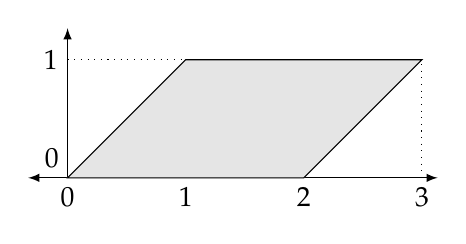
\begin{tikzpicture}
 		\draw[latex-latex] (-0.5,0) -- (4.7,0);
 		\draw[-latex] (0,0) node[below]{$0$} node[above, xshift=-0.2cm]{$0$}-- (0,1.9);
 		\draw[dotted] (0,1.5) node[left] {$1$}-- (4.5,1.5) -- (4.5,0);
 		\filldraw[black!10!white] (0,0) -- (1.5,1.5) -- (4.5,1.5) -- (3,0) -- cycle;
 		\draw (0,0) -- (1.5,1.5) -- (4.5,1.5) -- (3,0) -- cycle;
 		\draw (1.5,0) node[below] {$1$};
 		\draw (3,0) node[below] {$2$};
 		\draw (4.5,0) node[below] {$3$};
 	\end{tikzpicture}
 \end{center}
\begin{enumerate}[label=(\alph*)]
	\item Determine the value of $f\st_{X,Y}$ on the region shown
	\item Find $f\st_X$, the marginal pdf of $X$.
	\item Find the mean and variance of $X$.
	\item Find the conditional pdf of $Y$ given that $X=x$, for $0\leq x\leq 1$.
	\item Find the conditional pdf of $Y$ given that $X=x$, for $1\leq x\leq 2$.
	\item Find and sketch $\bbE[Y\mid X=x]$ as a function of $x$. Be sure to specify which range of $x$ this conditional expectation is well defined for.
\end{enumerate}
\end{problem}
\solve{
\begin{enumerate}[label=(\alph*)]
	\item The parallelogram has base length $2$ and height $1$. Therefore area of the parallel is $2\times 1$. Hence value of $f\st_{X,Y}(x,y)=\frac12$  on the region shown.
	\item For $0\leq x\leq 1$ $$f\st_X(x)=\int_0^xf\st_{X,Y}(x,y)dy=\int_0^x \frac12dy=\frac{x}2$$Now for  $1\leq x\leq 2$ $$f\st_X(x)=\int_0^1 f\st_{X,Y}(x,y)\; dy=\int_0^1\frac12\; dy=\frac12$$ And $2\leq x\leq 3$ $$f\st_X(x)=\int_{x-2}^1f\st_{X,Y}(x,y)dy=\int_x^1 \frac12dy=\frac{3-x}2$$Therefore $$f\st_X(x)=\begin{cases}
		\frac{x}2 & \text{when $0\leq x\leq 1$}\\
		\frac12 & \text{when $1\leq x\leq 2$}\\
		\frac{3-x}2 & \text{when $2\leq x\leq 3$}\\
		0 & \text{else}
	\end{cases}$$
\item \begin{align*}
	\bbE[X] & = \int_{-\infty}^{\infty} xf\st_X(x)dx\\
	& =\int_0^1\frac{x^2}{2}dx +\int_1^2 \frac{x}2dx+ \int_2^3\frac{x(3-x)}2dx\\
	& = \lt[\frac{x^3}6\rt]_0^1+\lt[\frac{x^2}{4}\rt]^2_1+\lt[\frac{3x^2}{4}-\frac{x^3}{6}\rt]_2^3\\
	& = \frac16+\frac34+\frac{7}{12}=\frac32
\end{align*}And \begin{align*}
\bbE[X^2] & = \int_0^1x^2f\st_X(x)dx\\
& = \int_0^1\frac{x^3}2dx+\int_1^2\frac{x^2}2dx+ \int_2^3\frac{x^2(1-x)}2dx\\
& = \lt[\frac{x^4}8\rt]_0^1+\lt[\frac{x^3}6\rt]_1^2+\lt[\frac{x^3}6-\frac{x^4}8\rt]_2^3\\
& = \frac18+\frac76+\frac{11}8=\frac83
\end{align*}Hence the variance will be $$\Var[X]=\bbE[X]^2-\bbE[X]^2=\frac83-\frac94=\frac5{12}$$
\item We have $$f\st_{Y\mid X}(y\mid X=x)=\frac{f\st_{X,Y}(x,y)}{f\st_{X}(x)}$$For $0\leq x\leq 1$ we have $$f\st_{Y\mid X}(y\mid X=x)=\frac{\frac12}{\frac{x}2}=\frac1x$$
\item For $1\leq x\leq 2$ we have $$f\st_{Y\mid X}(y\mid X=x)=\frac{\frac12}{\frac{1}2}=1$$
\item For $2\leq 3$ we have $$f\st_{Y\mid X}(y\mid X=x)=\frac{\frac{3-x}{2}}{\frac{1}2}=\frac1{3-x}$$Therefore we have $$f\st_{Y\mid X=x}(y)=\begin{cases}
	\frac1x & \text{when $0<x\leq 1$}\\
	1 & \text{when $1<x\leq 2$}\\
	\frac{1}{3-x} & \text{when $2<x\leq 3$}\\
	0 &\text{else}
\end{cases}$$Now if $0<x\leq 1$\begin{align*}
\bbE[Y\mid X=x] & = \int_{-\infty}^{\infty}yf\st_{Y\mid X}(y\mid x)dy\\
& = \int_0^x y\frac{1}xdy = \lt[\frac{y^2}{2x}\rt]_0^x=\frac{x^2}{2x}=\frac{x}2
\end{align*}
If $1<x\leq 2$ then \begin{align*}
	\bbE[Y\mid X=x] & = \int_{-\infty}^{\infty}yf\st_{Y\mid X}(y\mid x)dy\\
	& =  \int_0^1 y\cdot 1dy =\lt[\frac{y^2}2\rt]^1_0=\frac1{2}
\end{align*} If $2<x\leq 3$ \begin{align*}
\bbE[Y\mid X=x] & = \int_{-\infty}^{\infty}yf\st_{Y\mid X}(y\mid x)dy\\
& = \int_{x-2}^1\frac{y}{3-x}dy\\
& = \lt[\frac{y^2}{2(3-x)}\rt]^1_{2-x}=\frac1{2(3-x)}-\frac{(2-x)^2}{2(3-x)}=\frac{4x-3-x^2}{2(3-x)}=\frac{(x-3)(x-1)}{2(x-3)}=\frac{x-1}{2}
\end{align*}Hence we have $$\bbE[Y\mid X=x]=\begin{cases}
\frac{x}2 & \text{when $0<x\leq 1$}\\ \frac12 & \text{when $1<x\leq 2$}\\ \frac{x-1}{2} & \text{when $2<x\leq 3$}\\ 0 & \text{else}
\end{cases}$$
\end{enumerate}
}


%%%%%%%%%%%%%%%%%%%%%%%%%%%%%%%%%%%%%%%%%%%%%%%%%%%%%%%%%%%%%%%%%%%%%%%%%%%%%%%%%%%%%%%%%%%%%%%%%%%%%%%%%%%%%%%%%%%%%%%%%%%%%%%%%%%%%%%%
% Problem 6
%%%%%%%%%%%%%%%%%%%%%%%%%%%%%%%%%%%%%%%%%%%%%%%%%%%%%%%%%%%%%%%%%%%%%%%%%%%%%%%%%%%%%%%%%%%%%%%%%%%%%%%%%%%%%%%%%%%%%%%%%%%%%%%%%%%%%%%%

\begin{problem}{%problem statement 
	}{p6% problem reference text
	}
	Let $X,Y,Z$ be three jointly distributed random variables. Suppose \begin{enumerate}[label=(\roman*)]
		\item $X$ and $Y$ are independent
		\item $X$ and $Z$ are independent conditioned on $Y$
	\end{enumerate}
Prove or disprove the following claims:
 \begin{enumerate}[label=(\roman*)]
 	\item $X$ and $Y$ are independent conditioned on $Z$
 	\item $X$ and $Z$ are independent
 \end{enumerate}
\end{problem}
\solve{
Given that $X,Y$ are independent and $X,Z$ are independent conditioned on $Y$. Now \begin{align*}
	         & \bbP[X\cap Z\mid Y]=\bbP[X\mid Y]\bbP[Z\mid Y]                                                 \\
	\implies & \frac{\bbP[X\cap Z\cap Y]}{\bbP[Y]}=\frac{\bbP[X\cap Y]}{\bbP[Y]}\frac{\bbP[Z\cap Y]}{\bbP[Y]} \\
	\implies & \bbP[X\cap Y\cap Z]= \frac{\bbP[X]\bbP[Y]}{\bbP{[Y]}}\bbP[Y\cap Z]                             \\
	\implies & \bbP[X\cap Y\cap Z]=\bbP[X]\bbP[Y\cap Z]
\end{align*}
Now since $X,Y$ are independent $$\bbP[X\cap Y^c]=\bbP[X]-\bbP[X\cap Y]=\bbP[X]-\bbP[X]\bbP[Y]=\bbP[X](1-\bbP[Y])$$That means $X,Y^c$ is also independent. Therefore using the same process as above we get \begin{align*}
	         & \bbP[X\cap Z\mid Y^c]=\bbP[X\mid Y^c]\bbP[Z\mid Y^c]                                                       \\
	\implies & \frac{\bbP[X\cap Z\cap Y^c]}{\bbP[Y^c]}=\frac{\bbP[X\cap Y^c]}{\bbP[Y^c]}\frac{\bbP[Z\cap Y^c]}{\bbP[Y^c]} \\
	\implies & \bbP[X\cap Y^c\cap Z]= \frac{\bbP[X]\bbP[Y^c]}{\bbP{[Y^c]}}\bbP[Y^c\cap Z]                                 \\
	\implies & \bbP[X\cap Y^c\cap Z]=\bbP[X]\bbP[Y^c\cap Z]
\end{align*}Therefore we get \begin{align*}
\bbP[X\cap Z]& =\bbP[X\cap Y\cap Z]+\bbP[X\cap Y^c\cap Z]\\
& = \bbP[X]\bbP[Y\cap Z]+\bbP[X]\bbP[Y^c\cap Z]\\
& = \bbP[X](\bbP[Y\cap Z]+\bbP[Y^c\cap Z])\\
& = \bbP[X]\bbP[Z]
\end{align*}Hence we obtain $X,Z$ are independent. Now since $X,Z$ are independent we will derive that $X$ and $Y$ are independent conditioned on $Z$. \begin{align*}
& \bbP[X\cap Y\cap Z]=\bbP[X]\bbP[Y\cap Z]\\
\implies & \frac{\bbP[X\cap Y\cap Z]}{\bbP[Z]}=\frac{\bbP[X]\bbP[Y\cap Z]}{\bbP[Z]}\\
\implies & \bbP[X\cap Y\mid Z]=\frac{\bbP[X]\bbP[Z]}{\bbP[Z]}\bbP[Y\cap Z]\\
\implies & \bbP[X\cap Y\mid Z]=\frac{\bbP[X\cap Z]}{\bbP[Z]}\bbP[Y\cap Z]\\
\implies & \bbP[X\cap Y\mid Z]=\bbP[X\mid Z]\bbP[Y\mid Z]
\end{align*}
Therefore $X,Y$ are  independent conditioned on $Z$. 

Hence we have both results:  $X$,  $Y$ are independent conditioned on $Z$ and $X$, $Z$ are independent.
}\parinf

[I discussed the solution with Spandan]\parinn


%%%%%%%%%%%%%%%%%%%%%%%%%%%%%%%%%%%%%%%%%%%%%%%%%%%%%%%%%%%%%%%%%%%%%%%%%%%%%%%%%%%%%%%%%%%%%%%%%%%%%%%%%%%%%%%%%%%%%%%%%%%%%%%%%%%%%%%%
% Problem 7
%%%%%%%%%%%%%%%%%%%%%%%%%%%%%%%%%%%%%%%%%%%%%%%%%%%%%%%%%%%%%%%%%%%%%%%%%%%%%%%%%%%%%%%%%%%%%%%%%%%%%%%%%%%%%%%%%%%%%%%%%%%%%%%%%%%%%%%%

\begin{problem}{%problem statement 
	}{p7% problem reference text
	}
Let $X_1,X_2,\dots, X_n$ be independent, identically distributed random variables. Suppose their (common) marginal distribution function is $F\st_X$. Let $Y=\max(X_1,X_2,\dots, X_n)$ and $Z=\min (X_1,X_2,\dots, X_n)$. Find the distribution functions of $Y$ and $Z$. Assume $F\st_X$ has a density function $f\st_X$. Find the density functions of $Y,Z$ and $Y-Z$.
\end{problem}
\solve{
$Y=\max(X_1,X_2\dots, X_n)$. Hence for any $y$ $$Y\leq y\iff \max(X_1,\dots, X_n)\leq y\iff X_i\leq y\ \forall\ i\in[n]$$Suppose $F\st_Y$ is the distribution function of $Y$. Then $$F\st_Y(y)=\bbP[Y\leq y]=\bbP[\max(X_1,\dots, X_n)\leq y]=\bbP[X_1\leq y,X_2\leq y,\dots, X_n\leq y]=\prod_{i=1}^n\bbP[X_i\leq y]=F\st_X^n(y)$$Therefore $F\st_Y(y)=F\st_X^n(y)$. Hence density function of $Y$ is $f\st_Y(y)=nF\st_X^{n-1}(y)f\st_X(y)$

Now $Z=\min(X_1,X_2,\dots, X_n)$. Hence for any $z$ $$Z>z\iff \min(X_1,\dots, X_n)>z\iff X_i>z\ \forall\ i\in[n]$$Suppose $F\st_Z$ be the distribution function of $Z$. Then 
$$1-F\st_Z(z)=\bbP[Z>z]=\bbP[\min(X_1,\dots, X_n)>z]=\bbP[X_1> z,\dots, X_n>z]=\prod_{i=1}^n\bbP[X_i>z]=\lt(1-F\st_X(z)\rt)^n$$Hence $F\st_Z(z)=1-\lt(1-F\st_X(z)\rt)^n$. Hence density function of $ Z$ is $f\st_Z(z)=n\lt(1-F\st_X(z)\rt)^{n-1}f\st_X(z)$.

Now we will compute the density functions of $Y-Z$. First we will compute density function of $Y,Z$. Now $$F\st_{Y,Z}(y,z)=\bbP[Y\leq y, Z\leq z]=\bbP[Y\leq y]-\bbP[Y\leq y,Z>z]=F\st_X(y)^n-\bbP[Y\leq y,Z>z]$$Hence if $y< z$ then $\bbP[Y\leq y,Z>z]=0$ otherwise when $y\geq z$ we have $$\bbP[Y\leq y,Z>z]=\lt(F\st_X(y)-F\st_X(z)\rt)^n$$Therefore we have $$F\st_{Y,Z}(y,z)=\begin{cases}
	F\st_X^n(y)-\lt(F\st_X(y)-F\st_X(z)\rt)^n & \text{when }z\leq y\\
	F\st_X^n(y) &\text{else}
\end{cases}$$Therefore we get the density function $$f\st_{Y,Z}(y,z)=\frac{\partial^2}{\partial y\partial z}F\st_{Y,Z}(y,z)=\begin{cases}
n(n-1)\lt(F\st_X(y)-F\st_X(z)\rt)^{n-2}f\st_X(y)f\st_X(z) & \text{when }z\leq y\\
0 & \text{else}
\end{cases}$$Now take the random variables $U=Y-Z$ and $V=Z$. Then we replace variables by $y=u+v$ and $z=v$ when $z\leq y$ or $u\geq 0$. Hence $$\mcJ(u,v)=\detmat{\deld{y}{u} & \deld{z}{u}\\[4mm] \deld{y}{v} & \deld{z}{v}}=\detmat{1 & 0 \\ 1 & 1}=1$$Hence when $u\geq 0$ $$f\st_{U,V}(u,v)=f\st_{Y,Z}(y(u,v), z(u,v))\; |\mcJ|=f\st_{Y,Z}(y(u,v), z(u,v))=n(n-1)\lt(F\st_X(u+v)-F\st_X(v)\rt)^{n-2}f\st_X(u+v)f\st_X(v)$$Therefore $$f\st_U(u)=\begin{cases}
\int_{-\infty}^{\infty}n(n-1)\lt(F\st_X(u+v)-F\st_X(v)\rt)^{n-2}f\st_X(u+v)f\st_X(v)\; dv & \text{when $u\geq 0$}\\ 0 & \text{else}
\end{cases}$$
}\parinf

[I discussed with Spandan]


%%%%%%%%%%%%%%%%%%%%%%%%%%%%%%%%%%%%%%%%%%%%%%%%%%%%%%%%%%%%%%%%%%%%%%%%%%%%%%%%%%%%%%%%%%%%%%%%%%%%%%%%%%%%%%%%%%%%%%%%%%%%%%%%%%%%%%%%
% Problem 8
%%%%%%%%%%%%%%%%%%%%%%%%%%%%%%%%%%%%%%%%%%%%%%%%%%%%%%%%%%%%%%%%%%%%%%%%%%%%%%%%%%%%%%%%%%%%%%%%%%%%%%%%%%%%%%%%%%%%%%%%%%%%%%%%%%%%%%%%

\begin{problem}{%problem statement 
		[H] Problem 1.31: Transformation of densities
	}{p8% problem reference text
	}
	Let $U$ and $V$ have the joint pdf: $$f\st_{UV}(u,v)=\begin{cases}
		c(u-v)^2 & 0\leq u,v\leq 1\\ 0 & \text{else}
	\end{cases}$$for some constant $c$.
\begin{enumerate}[label=(\alph*)]
	\item Find the constant $c$
	\item Suppose $X=U^2$ and $Y=U^2V^2$. Describe the joint pdf $f\st_{X,Y}(x,y)$ of $X$ and $Y$. Be sure to indicate where the joint pdf is zero.
\end{enumerate}
\end{problem}
\solve{
\begin{enumerate}[label=(\alph*)]
	\item We know $\int\limits_{-\infty} ^{\infty}  \int\limits_{-\infty}^{\infty}  f\st_{UV}(u,v)\; dudv=1$. Therefore we have\begin{align*}
		\int_{-\infty} ^{\infty}  \int_{-\infty}^{\infty}  f\st_{UV}(u,v)\; dudv &= \int_0^1\int_0^1c(u-v)^2\; dudv\\
		& = \int_0^1c\lt[\int_0^1(x^2-2xy+y^2)\;dx\rt]\;dy\\
		& =\int_0^1c\lt[\frac{x^3}{3}-x^2y+y^2x\rt]_0^1\;\\
		& = c\int_0^1\lt[\frac13-y+y^2\rt]\;dy\\
		& = c\lt[\frac{y}3-\frac{y^2}2+\frac{y^3}3\rt]_0^1 = c\lt[\frac13-\frac12+\frac13\rt]=\frac{c}6
	\end{align*}Therefore we have $\frac{c}{6}=1\iff c=6$.
\item $X=U^2\implies U=\sqrt{X}$. Now $Y=U^2V^2\implies  \sqrt{Y}=UV\implies V=\sqrt{\frac{Y}{X}}$. Since $0\leq u,v\leq 1$ take $0\leq y\leq x\leq 1$.  So take $u=\sqrt{x}$ and $v=\sqrt{\frac{y}{x}}$.   Therefore for  $0<y\leq x\leq 1$ $$\mcJ(x,y)=\detmat{\deld{u}{x} & \deld{v}{x}\\[4mm] \deld{u}{y} & \deld{v}{y}}=\detmat{ \frac1{2\sqrt{x}} & -\frac12{x^{-\frac32}}  {\sqrt{y}}\\[4mm]  0 & \frac1{2\sqrt{xy}}}=\frac1{4x\sqrt{y}}$$Hence we have $$f\st_{X,Y}(x,y)=f\st_{U,V}(u(x,y), v(x,y))\; |\mcJ|=f\st_{U,V}\lt(\sqrt{x},\sqrt{\frac{y}{x}}\rt)\frac1{4x\sqrt{y}}$$Therefore for $0<y\leq x\leq 1$ we have $$f\st_{X,Y}(x,y)=\lt(\sqrt{x}-\sqrt{\frac{y}{x}}\rt)^2\frac{1}{4x\sqrt{y}}=\lt(x-2\sqrt{y}+\frac{y}{x}\rt)\frac{1}{4x\sqrt{y}}=\frac1{4\sqrt{y}}-\frac{1}{2x}+\frac{\sqrt{y}}{4x^2}$$Hence $$f\st_{X,Y}(x,y)=\begin{cases}
	\frac1{4\sqrt{y}}-\frac{1}{2x}+\frac{\sqrt{y}}{4x^2} & 0<y\leq x\leq 1\\
	0& \text{else}
\end{cases}$$
\end{enumerate}
}



%%%%%%%%%%%%%%%%%%%%%%%%%%%%%%%%%%%%%%%%%%%%%%%%%%%%%%%%%%%%%%%%%%%%%%%%%%%%%%%%%%%%%%%%%%%%%%%%%%%%%%%%%%%%%%%%%%%%%%%%%%%%%%%%%%%%%%%%
% Problem 9
%%%%%%%%%%%%%%%%%%%%%%%%%%%%%%%%%%%%%%%%%%%%%%%%%%%%%%%%%%%%%%%%%%%%%%%%%%%%%%%%%%%%%%%%%%%%%%%%%%%%%%%%%%%%%%%%%%%%%%%%%%%%%%%%%%%%%%%%

\begin{problem}{%problem statement 
		[H] Problem 1.33: Transformation of joint densities
	}{p9% problem reference text
	}
	Assume $X$ and $Y$ are independent, each with the exponential pdf with parameter $\lm>0$. Let $W=X-Y$ and $Z=X^2+X-Y$. Find the joint pdf of $(W,Z)$. Be sure to specify its support (i.e. where it is not zero).
\end{problem}
\solve{$W=X-Y$. $Z=X^2+X-Y=X^2+W\iff X^2=Z-W\implies X=\sqrt{Z-W}$. Therefore $Y=X-W=\sqrt{Z-W}-W$. So we take $x=\sqrt{z-w}$ and $y=\sqrt{z-w}-w$. Then for $z\geq w$ we have$$\mcJ(w,z)=\detmat{\deld{x}{w} & \deld{y}{w}\\[4mm] \deld{x}{z} & \deld{y}{z}}= \detmat{-\frac1{2\sqrt{z-w}} & -\frac1{2\sqrt{z-w}}-1\\[4mm] \frac{1}{2\sqrt{z-w}} & \frac{1}{2\sqrt{z-w}} }=-\frac1{2\sqrt{z-w}} \frac{1}{2\sqrt{z-w}}+\lt[ \frac1{2\sqrt{z-w}}+1 \rt] \frac{1}{2\sqrt{z-w}}=\frac1{2\sqrt{z-w}}$$Hence$$f\st{W,Z}(w,z)=f\st_{X,Y}(x(w,z), y(w,z))\;|\mcJ|=f\st_{X}(x(w,z))\; f\st_Y( y(w,z))\; |\mcJ|$$Now $X,Y$ are independent and both of them are exponential random variables with parameter $\lm>0$. Hence $f\st_X(x)=\lm e^{-\lm x}$ and $f\st_Y(y)=\lm e^{-\lm y}$. Therefore $$f\st_X(x(w,z))=\lm e^{-\lm \sqrt{z-w}}\qquad f\st_Y(y(z,w))=\lm e^{-\lm (\sqrt{z-w}-w)}$$Therefore $$f\st_{W,Z}(w,z)=\lm e^{-\lm \sqrt{z-w}}\; \lm e^{-\lm (\sqrt{z-w}-w)}\; \frac1{2\sqrt{z-w}}=\frac{\lm^2e^{-\lm (2\sqrt{z-w}-w)}}{2\sqrt{z-w}}$$when $z\geq w$. Hence we have $$f\st_{W,Z}(w,z)=\begin{cases}
		\frac{\lm^2e^{-\lm (2\sqrt{z-w}-w)}}{2\sqrt{z-w}} & z\geq w\\ 0 & \text{else}
	\end{cases}$$
}

\newpage

%%%%%%%%%%%%%%%%%%%%%%%%%%%%%%%%%%%%%%%%%%%%%%%%%%%%%%%%%%%%%%%%%%%%%%%%%%%%%%%%%%%%%%%%%%%%%%%%%%%%%%%%%%%%%%%%%%%%%%%%%%%%%%%%%%%%%%%%
% Problem 10
%%%%%%%%%%%%%%%%%%%%%%%%%%%%%%%%%%%%%%%%%%%%%%%%%%%%%%%%%%%%%%%%%%%%%%%%%%%%%%%%%%%%%%%%%%%%%%%%%%%%%%%%%%%%%%%%%%%%%%%%%%%%%%%%%%%%%%%%

\begin{problem}{%problem statement 
		[H] Problem 1.35: Conditional densities and expectations
	}{p10% problem reference text
	}
	Suppose the random variables $X$ and $Y$ have the joint pdf:$$f\st_{XY}(u,v)=\begin{cases}
		4u^2 & 0<v<u<1\\ 0& \text{elsewhere}
	\end{cases}$$\begin{enumerate}[label=(\alph*)]
	\item Find $\bbE[XY]$
	\item Find $f\st_Y(v)$. Be sure to specify it for all values of $v$.
	\item Find $f\st_{X\mid Y}(u\mid v)$. Be sure to specify where it is undefined and where it is zero.
	\item Find $\bbE[X^2\mid Y=v]$ for $0<v<1$.
\end{enumerate}
\end{problem}
\solve{
\begin{enumerate}[label=(\alph*)]
	\item \begin{align*}
		\bbE[XY] & = \int_{-\infty}^{\infty}\int_{-\infty}^{\infty}uv\; f\st_{X,Y}(u,v)\; dudv\\
		& = \int_0^1\int_0^u uv\cdot 4u^2\; dudv\\
		& = \int_0^1\int_0^u 4u^3v\; dudv\\
		& = \int_0^1 \lt[ 2u^3v^2  \rt]_0^u\; dv\\
		& = \int_0^1 2u^5\; du\\
		& = \lt[\frac{2u^6}{6}\rt]_0^1=\frac13
	\end{align*}
\item Now for $y>0$ we have $$f\st_Y(v)=\int_{-\infty}^{\infty}f\st_{X,Y}(u,v)\; du = \int_v^14u^2 \; du=\lt[\frac{4u^3}3\rt]_v^1=\frac{4(1-v^3)}{3}$$ Hence we have $$f\st_Y(v)=\begin{cases}
	\frac{4(1-v^3)}{3} & \text{when }v>0\\
	0 & \text{else}
\end{cases}$$
\item When $0<v<u<1$ we have $$f\st_{X\mid Y}(u\mid v)=\frac{f\st_{X,Y}(u,v)}{f\st_Y(v)}=\frac{4u^2}{\frac{4(1-v^3)}{3}}=\frac{3u^2}{1-v^3}$$Therefore $$f\st_{X\mid Y}(u\mid v)=\begin{cases}
	\frac{3u^2}{1-v^3} & \text{when $0<v<u<1$}\\ 0 & \text{else}
\end{cases}$$
\item \begin{align*}
	\bbE[X^2 \mid Y=v]& =\int_{-\infty}^{\infty} u^2 f\st_{X\mid Y}(u\mid v)\; du\\
	& = \int_v^1 \frac{3u^4}{1-v^3}du\\
	 & = \lt[  \frac{3u^5}{5(1-v^3)}\rt]_v^1\\
	 & = \frac{3(1-v^5)}{5(1-v^3)}
\end{align*}
\end{enumerate}
}

\end{document}
